\newcommand{\mpgvsweight}[1]{
    \begin{tikzpicture}
        \begin{axis}[
            height=7cm,
            width=10cm,
            xlabel=$x$ (horsepower),
            ylabel=$y$ (mpg),
            ytick pos=left,
            xtick pos=bottom,
            xmin=30,
            xmax=245,
            ymin=6,
            ymax=51
        ]

            \addplot[
                only marks,
                cyan,
                opacity=0.5
            ] table [
                col sep=comma,
                x=horsepower,
                y=mpg
            ] {data/Auto.csv};

            \ifnum#1=1
                \draw[very thick, red] (axis cs: 30, 39-0.157*30) -- (axis cs: 245, 39-0.157*245);
                \node[text=red] at (axis cs: 180, 42) {
                    $\hat{f}(x) = 39 - 0.157x$
                };
            \fi
            \ifnum#1=2
                \addplot[very thick, red, domain=30:245, samples=1000] {0.0012*x^2-0.46*x+56};
                \node[text=red] at (axis cs: 180, 42) {
                    $\hat{f}(x) = 56+0.0012x^2-0.46x$
                };
            \fi
        \end{axis}
    \end{tikzpicture}
}

\newcommand{\modeltypes}{
    \begin{tikzpicture}
        \begin{axis}[
            height=5cm,
            width=10cm,
            xlabel=$x$ (horsepower),
            ylabel=$y$ (mpg),
            ytick pos=left,
            xtick pos=bottom,
            xmin=30,
            xmax=245,
            ymin=6,
            ymax=51
        ]

        \addplot[
            only marks,
            cyan,
            opacity=0.5
        ] table [
            col sep=comma,
            x=horsepower,
            y=mpg
        ] {data/Auto.csv};

        \draw[very thick, red] (axis cs: 30, 39-0.157*30) -- (axis cs: 245, 39-0.157*245);
        \node[align=left] at (axis cs: 180, 35) {
            $
            \begin{aligned}
                {\color{red}\hat{f}(x) }&{\color{red}= 39 - 0.157x}\\
                {\color{teal}\hat{f}(x) }&{\color{teal}= \ldots}\\
            \end{aligned}
            $
        };

        \addplot[very thick, teal, smooth] coordinates {
            (6.0, 243.2069751806266)
            (15.958333333333334, 118.86132183998052)
            (25.916666666666668, 55.54830308937471)
            (35.875, 33.03657403682814)
            (45.833333333333336, 31.094789790600284)
            (55.79166666666667, 32.62203312809545)
            (65.75, 32.322995894942245)
            (75.70833333333334, 26.789726618159705)
            (85.66666666666667, 25.56443372228785)
            (95.625, 23.411114113578773)
            (105.58333333333334, 21.972291293527256)
            (115.54166666666667, 22.0202279029072)
            (125.5, 19.623191768387127)
            (135.45833333333334, 17.796535374305538)
            (145.41666666666669, 15.42464063855285)
            (155.375, 13.83975395598323)
            (165.33333333333334, 13.58266973340266)
            (175.29166666666669, 14.577234897250934)
            (185.25, 13.44873671948327)
            (195.20833333333334, 11.13569858732588)
            (205.16666666666669, 10.948027264126887)
            (215.125, 12.746078206932541)
            (225.08333333333334, 14.710541046885707)
            (235.04166666666669, 16.775438769652766)
            (245.0, 18.301538120974897)
        };

        \end{axis}
    \end{tikzpicture}
}


\newcommand{\tradeoffplot}[1]{
    \definecolor{full}{HTML}{ef476f}
    \definecolor{bias}{HTML}{26547c}
    \definecolor{variance}{HTML}{06d6a0}
    \definecolor{train}{HTML}{ffd166}

    \begin{tikzpicture}
        \begin{axis}[
            height=6cm,
            width=9cm,
            ymajorticks=false,
            xmajorticks=false,
            ylabel=Model error,
            xlabel=Flexibility,
            axis lines=left,
            xmin=0,
            xmax=1,
            ymin=0,
            ymax=2.5,
            clip=false
        ]
            \node[] at (axis cs: 1.34, 2.9) {};

            \ifnum#1>0
                \draw[dotted] (axis cs: 0.1, 0) -- (axis cs: 0.1, 2.5);
                \node[anchor=south, align=center, font=\footnotesize\linespread{0.9}\selectfont] at (axis cs: 0.1, 2.5) {
                    Simple\\model
                };
                \addplot[
                    only marks,
                    mark options={
                        draw=black,
                        fill=bias,
                        scale=2
                    }
                ] coordinates {
                    (0.1, 0.5)
                    (1.05, 2.4)
                };
                \node[anchor=west] at (axis cs: 1.065, 2.4) {
                    Bias
                };

                \addplot[
                    only marks,
                    mark options={
                        draw=black,
                        fill=variance,
                        scale=2
                    }
                ] coordinates {
                    (0.1, 0.01114)
                    (1.05, 2.2)
                };
                \node[anchor=west] at (axis cs: 1.065, 2.2) {
                    Variance
                };
            \fi
            \ifnum#1>1
                \draw[dotted] (axis cs: 0.75, 0) -- (axis cs: 0.75, 2.5);
                \node[anchor=south, align=center, font=\footnotesize\linespread{0.9}\selectfont] at (axis cs: 0.75, 2.5) {
                    Complex\\model
                };
                \addplot[
                    only marks,
                    mark options={
                        draw=black,
                        fill=bias,
                        scale=2
                    }
                ] coordinates {
                    (0.75, 0.117)
                };

                \addplot[
                    only marks,
                    mark options={
                        draw=black,
                        fill=variance,
                        scale=2
                    }
                ] coordinates {
                    (0.75, 0.2873)
                };
            \fi
            \ifnum#1>2
                \addplot[
                    bias,
                    very thick,
                    domain=0:1,
                    samples=100
                ] {(1/(x+0.1))/10};
                \addplot[
                    variance,
                    very thick,
                    domain=0:1,
                    samples=100
                ] {(exp(x*5))/148};
            \fi
            \ifnum#1>3
                \draw[dashed] (axis cs: 0, 1.2) -- (axis cs: 1, 1.2);
                \node[anchor=west, align=left, font=\footnotesize\linespread{0.9}\selectfont] at (axis cs: 1, 1.2) {
                    Irreducible\\error
                };
            \fi
            \ifnum#1>4
                \addplot[
                    full,
                    very thick,
                    domain=0:1,
                    samples=100
                ] {((1/(x+0.1))/10) + ((exp(x*5))/148) + 1.2};

                \addplot[
                    only marks,
                    mark options={
                        draw=black,
                        fill=full,
                        scale=2
                    }
                ] coordinates {
                    (0.1, 1.71114)
                    (0.75, 1.6043)
                    (1.05, 2)
                };
                \ifnum#1<6
                    \node[anchor=west] at (axis cs: 1.065, 2) {
                        Total
                    };
                \fi
            \fi
            \ifnum#1>5
                \addplot[
                    train,
                    very thick,
                    domain=0:1,
                    samples=100
                ] {((1/(x+0.1))/10) + 1.2};

                \node[anchor=west] at (axis cs: 1.065, 2) {
                    Total (test)
                };

                \addplot[
                    only marks,
                    mark options={
                        draw=black,
                        fill=train,
                        scale=2
                    }
                ] coordinates {
                    (0.1, 1.7)
                    (0.75, 1.317)
                    (1.05, 1.8)
                };
                \node[anchor=west] at (axis cs: 1.065, 1.8) {
                    Total (train)
                };
            \fi

        \end{axis}
    \end{tikzpicture}
}

\begin{frame}{Recap}
    \begin{tikzpicture}
        \node[] at (-5.25, -3.5) {};
        \node[] at (5.25, 3.5) {};

        \visible<1-4>{
            \node[anchor=west, text width=10cm] at (-5, 0) {
                \textbf{What is statistical learning?}
                \begin{itemize}
                    \item<2-> \underline{Inferentiental view:} \alert<4>{Finding a function $\hat{f}(X)$} that describes the relationship between some input variables $X$ and an output variable $y$.
                    \item<3->{\underline{Predictive view:} \alert<4>{Finding a function $\hat{f}(X)$} that, when given a new set of inputs $X$, allows us to predict an output $y$.}
                \end{itemize}
            };
        }
        \visible<5>{
            \node[] at (0, 0) {
                \mpgvsweight{0}
            };
        }
        \visible<6>{
            \node[] at (0, 0) {
                \mpgvsweight{1}
            };
        }
        \visible<7>{
            \node[] at (0, 0) {
                \mpgvsweight{2}
            };
        }
        \visible<8>{
            \node[inner sep=0pt, draw=black, anchor=west] (x1) at (-5.25, 2.5) {
                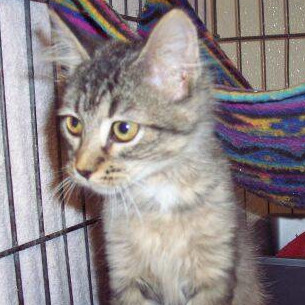
\includegraphics[width=1cm]{data/cats_and_dogs/cat.2.jpg}
            };
            \node[inner sep=0pt, draw=black] (x2) at ($ (x1) - (0, 1.5) $) {
                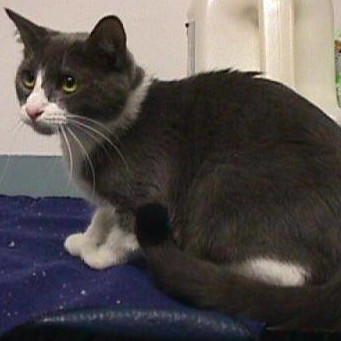
\includegraphics[width=1cm]{data/cats_and_dogs/cat.0.jpg}
            };
            \node[inner sep=0pt, draw=black] (x3) at ($ (x1) - (0, 3) $) {
                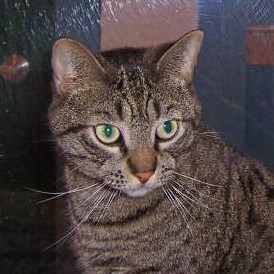
\includegraphics[width=1cm]{data/cats_and_dogs/cat.1.jpg}
            };
            \node[inner sep=0pt, draw=black] (x3) at ($ (x1) - (0, 4.5) $) {
                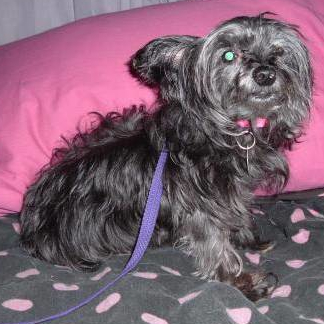
\includegraphics[width=1cm]{data/cats_and_dogs/dog.0.jpg}
            };

            \node[inner sep=0pt, draw=black] (x5) at ($ (x1) - (-1.25, 0.75) $) {
                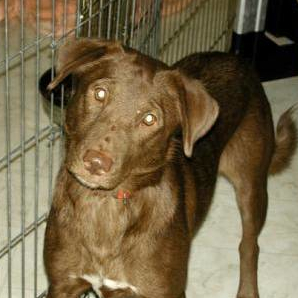
\includegraphics[width=1cm]{data/cats_and_dogs/dog.1.jpg}
            };
            \node[inner sep=0pt, draw=black] (x6) at ($ (x1) - (-1.25, 2.25) $) {
                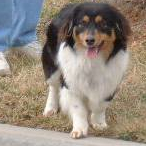
\includegraphics[width=1cm]{data/cats_and_dogs/dog.2.jpg}
            };
            \node[inner sep=0pt, draw=black] (x7) at ($ (x1) - (-1.25, 3.75) $) {
                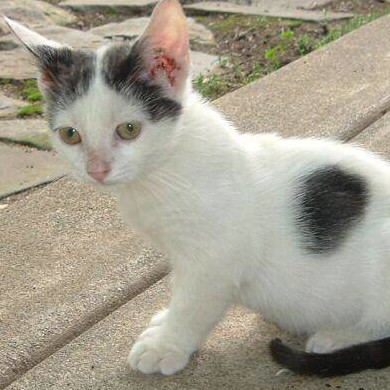
\includegraphics[width=1cm]{data/cats_and_dogs/cat.3.jpg}
            };

            \node[align=center, font=\scriptsize, draw=black] (sm) at ($ (x1) + (3.5, -0.55) $) {
                Supervised\\model
            };

            \draw[-stealth, gray!50, line width=3pt] (x6) to [in=270, out=0] (sm);
            \draw[-stealth, gray!50, line width=3pt] (sm) -- ($ (sm.east) + (1.1, 0) $);

            \node[inner sep=0pt, draw=black] (y1) at ($ (sm.center) + (5, 0.5) $) {
                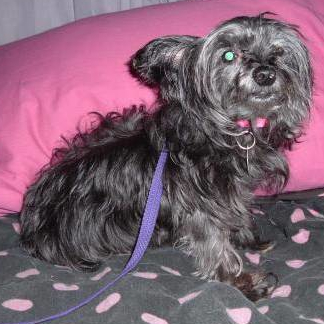
\includegraphics[width=1cm]{data/cats_and_dogs/dog.0.jpg}
            };
            \node[anchor=west, inner sep=0pt, draw=black] (y2) at (y1.east) {
                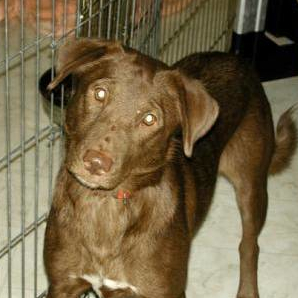
\includegraphics[width=1cm]{data/cats_and_dogs/dog.1.jpg}
            };
            \node[anchor=north, inner sep=0pt, draw=black] at (y1.south) {
                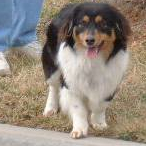
\includegraphics[width=1cm]{data/cats_and_dogs/dog.2.jpg}
            };

            \node[inner sep=0pt, draw=black] (y4) at ($ (sm) + (2.5, 0.5) $) {
                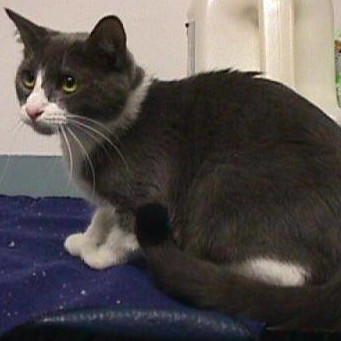
\includegraphics[width=1cm]{data/cats_and_dogs/cat.0.jpg}
            };
            \node[anchor=west, inner sep=0pt, draw=black] (y5) at (y4.east) {
                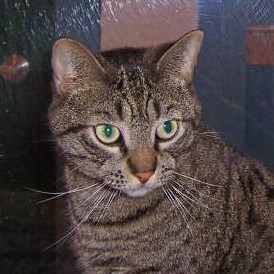
\includegraphics[width=1cm]{data/cats_and_dogs/cat.1.jpg}
            };
            \node[anchor=north, inner sep=0pt, draw=black] (y6) at (y4.south) {
                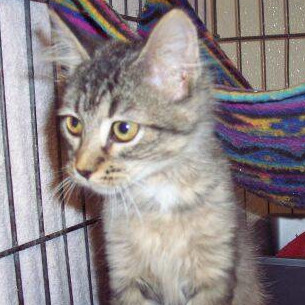
\includegraphics[width=1cm]{data/cats_and_dogs/cat.2.jpg}
            };
            \node[anchor=north, inner sep=0pt, draw=black] (y7) at (y5.south) {
                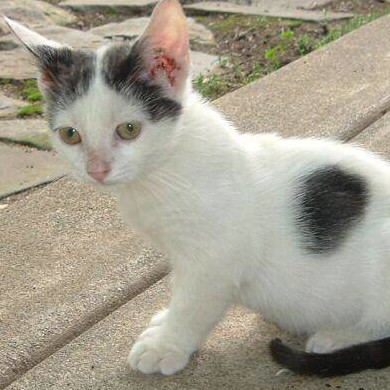
\includegraphics[width=1cm]{data/cats_and_dogs/cat.3.jpg}
            };

            \node[anchor=south, text depth=0] at ($ (y1.north)!0.5!(y2.north) $) {
                Dogs
            };
            \node[anchor=south, text depth=0] at ($ (y4.north)!0.5!(y5.north) $) {
                Cats
            };

            \node[align=center, font=\scriptsize, draw=black] (um) at ($ (x1) + (3.5, -3.95) $) {
                Unsupervised\\model
            };

            \draw[-stealth, gray!50, line width=3pt] (x6) to [in=90, out=0] (um);
            \draw[-stealth, gray!50, line width=3pt] (um) -- ($ (um.east) + (1.1, 0) $);

            \node[inner sep=0pt, draw=black] at ($ (um.center) + (6, 0.55) $) {
                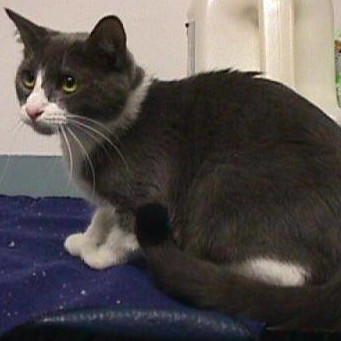
\includegraphics[width=1cm]{data/cats_and_dogs/cat.0.jpg}
            };
            \node[inner sep=0pt, draw=black] at ($ (um.center) + (5.95, -0.65) $) {
                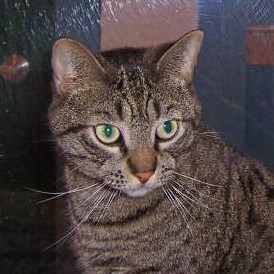
\includegraphics[width=1cm]{data/cats_and_dogs/cat.1.jpg}
            };
            \node[inner sep=0pt, draw=black] at ($ (um.center) + (4.8, 0.4) $) {
                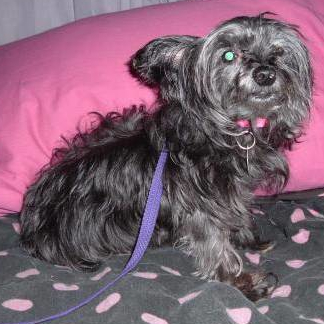
\includegraphics[width=1cm]{data/cats_and_dogs/dog.0.jpg}
            };
            \node[inner sep=0pt, draw=black] at ($ (um.center) + (4.7, -0.7) $) {
                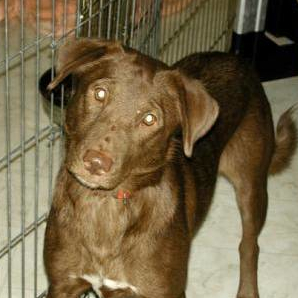
\includegraphics[width=1cm]{data/cats_and_dogs/dog.1.jpg}
            };

            \node[inner sep=0pt, draw=black] at ($ (um.center) + (2.7, 1.2) $) {
                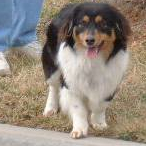
\includegraphics[width=1cm]{data/cats_and_dogs/dog.2.jpg}
            };
            \node[inner sep=0pt, draw=black] at ($ (um.center) + (2.55, 0) $) {
                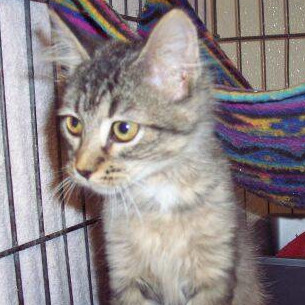
\includegraphics[width=1cm]{data/cats_and_dogs/cat.2.jpg}
            };
            \node[inner sep=0pt, draw=black] at ($ (um.center) + (2.65, -1.1) $) {
                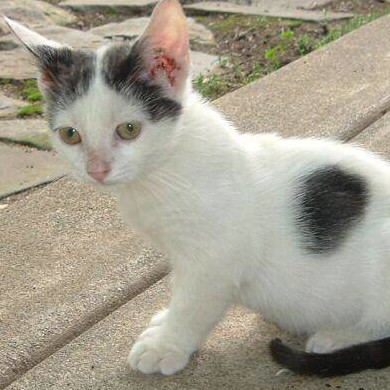
\includegraphics[width=1cm]{data/cats_and_dogs/cat.3.jpg}
            };
            \node[] at ($ (um.center) + (2.65, -1.87) $) {
                Cluster 1
            };
            \node[] at ($ (um.center) + (5.35, -1.45) $) {
                Cluster 2
            };
        }
        \visible<9>{
            \draw[dashed] (0, -3.5) -- (0, 3.5);
            \node[anchor=north] at (-2.675, 3.5) {\textbf{Regression}};
            \node[anchor=north] at (2.675, 3.5) {\textbf{Classification}};

            \node[ampersand replacement=\&, inner sep=0pt] (regdata) at (-2.675, 1) {
                \begin{tabular}{|c|}
                    \hline
                    $\boldsymbol{y}$\\
                    \hline
                    18\\
                    15\\
                    18\\
                    16\\
                    17\\
                    \hline
                \end{tabular}
            };
            \node[text width=5cm, align=flush center, font=\small\linespread{0.9}\selectfont, anchor=north] at (-2.675, -2.1) {
                The predictive target $y$ is a \textit{continuous} (or \textit{quantitative}) variable.
            };

            \node[ampersand replacement=\&, inner sep=0pt] (classdata) at (2.675, 1) {
                \begin{tabular}{|c|}
                    \hline
                    $\boldsymbol{y}$\\
                    \hline
                    cat\\
                    cat\\
                    dog\\
                    cat\\
                    dog\\
                    \hline
                \end{tabular}
            };
            \node[text width=5cm, align=flush center, font=\small\linespread{0.9}\selectfont, anchor=north] at (2.675, -2.1) {
                The predictive target $y$ is a \textit{categorical} (or \textit{qualitative}) variable.
            };
        }
        \visible<10>{
            \node[] at (0, 1.3) {
                \modeltypes
            };
            \node[text width=10.5cm] at (0, -2.2) {
                \begin{itemize}
                    \item \textbf{Parametric models} The function ${\color{red}\hat{f}(X)}$ is relatively simple and can be described by a small number of parameters.
                    \begin{itemize}
                        \item Linear regression: $\hat{f}(X) = \beta_0 + \beta_1x$
                    \end{itemize}
                    \item \textbf{Non-parametric models} The function ${\color{teal}\hat{f}(X)}$ is more complex and often relies directly on the data.
                \end{itemize}
            };
        }
        \visible<11>{
            \node[] at (0, 0) {
                \tradeoffplot{3}
            };
        }
        \visible<12>{
            \node[] at (0, 0) {
                \tradeoffplot{6}
            };
        }
    \end{tikzpicture}
\end{frame}
